\chapter{Implementation and Performance Analysis}

The core implementation is purposed at the official repository of the MLANN paper by Professor Savchenko. The algorithm is already implemented in \textit{C++} and Caffe by Professor Savchenko and is available via \href{https://github.com/HSE-asavchenko/HSE_FaceRec/tree/master/src}{this} link. I've also provided the \textit{C++} implementation in the directory of this project. In this section, we'll analyze the implementation of MLANN method using Tensorflow and OpenCV in Python.

\section{The Architecture}
Figure 3.1 illustrates the overall architecture of implementation.
\begin{figure}[!h]\centering
	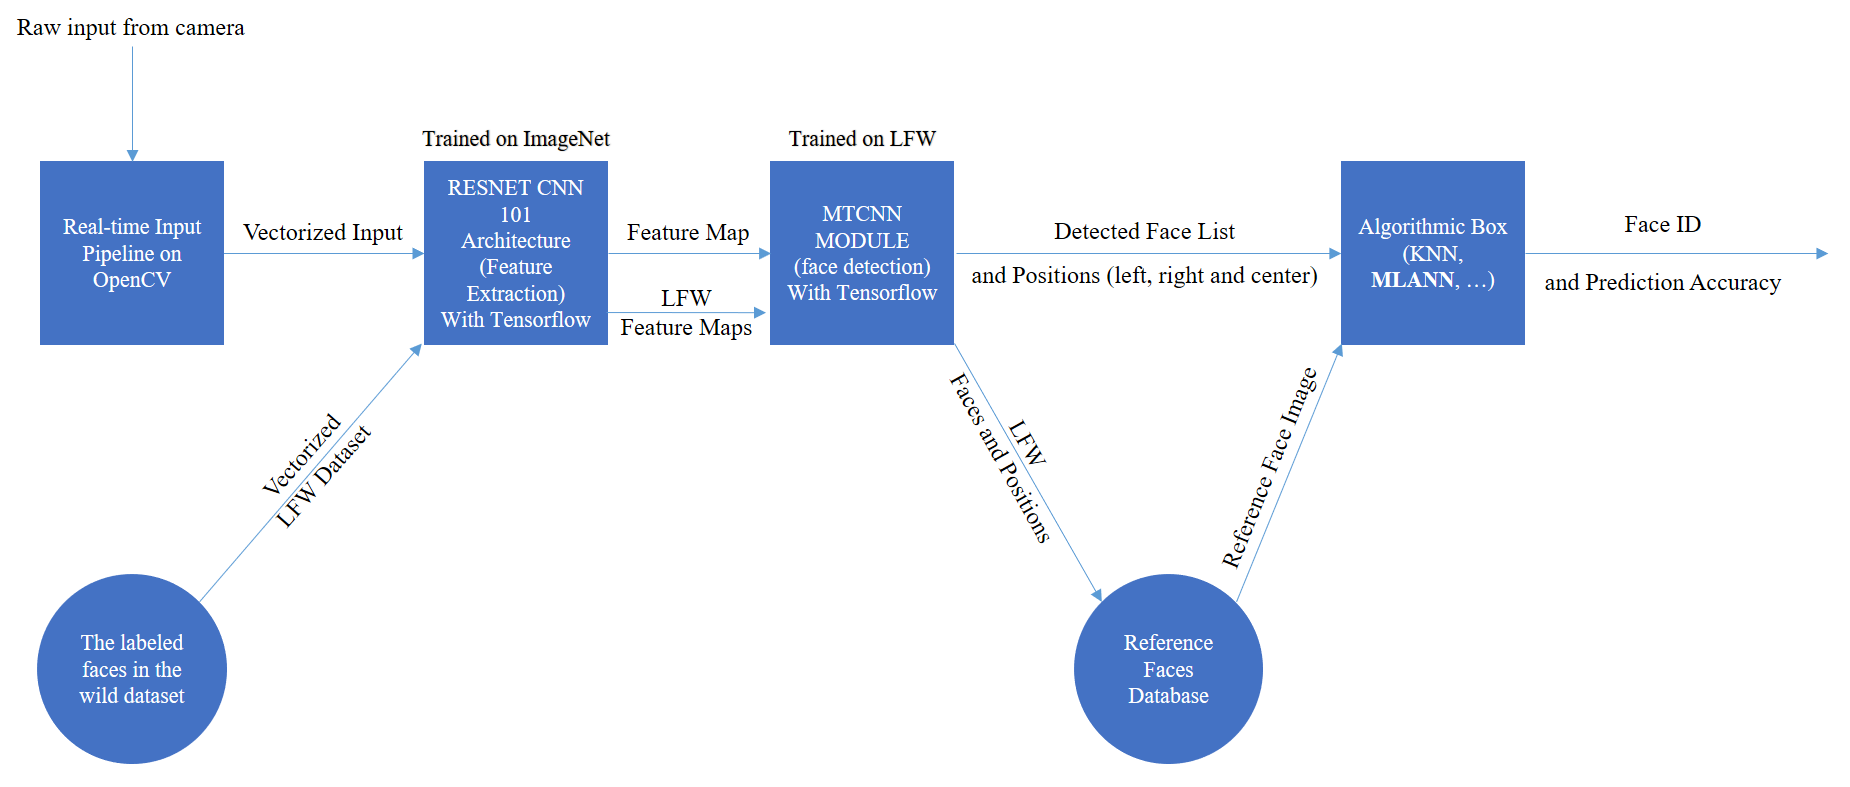
\includegraphics[width=1.1\textwidth]{diagram.PNG}
	\caption{The architecture of real-time face recognition system.}
	\label{pl1}
\end{figure}